% Please keep it to 80 columns, no tabs, no trailing whitespace
% and no Windows line endings (\r\n)
\documentclass[10pt,a4paper,oneside]{report}
\usepackage[utf8]{inputenc}
\usepackage{graphicx}
\usepackage{lscape}
\usepackage{float}
\usepackage{pdfpages}
\usepackage{graphics}
%% \usepackage{tabularx}
\usepackage{tabularx}
\begin{document}
\title{Group 8 Integrated Project Proposal\\Project Name Here}

% Names in alphabetical order.
% The mark is for the proposal part.
\author{
  Chen Guangyu (20\%)\\
  Kowalczyk Mateusz (20\%)\\
  Luff Katie (20\%)\\
  Sampson Robert (20\%)\\
  Singh Aman (20\%)\\ }
%\date{}
\maketitle
\section*{Background}
We are planning to develop a Bath University map application for mobile phone users. The main purpose that the application will serve is to guide the user to a building using a set of instructions. It will be integrated with a GPS to reduce the hassle of initial configuration. This system will be used to leverage further map functionality, such as finding various services available on campus.
We believe there is a gap in the market for this, as there is currently no route planning system around campus. There are four times during the year where students struggle to get to their destination: start of the year, middle of the year when timetables change and both exam periods which are often taken place in unfamiliar buildings. We believe that this application will help students settle into university life quicker, as well as helping to take away any unnecessary stress around exam periods.

\section*{Research}
\subsubsection*{Google Maps \& Bing}
For our domain research we looked into Google Maps as its key feature is also a path finder. Some good features that we are going to consider in our project is that is has multiple paths that you can choose from between two points. This is good as the maps don't take into account how busy the routes are so a longer distance may take less time. Another good aspect of the system is that you can have multiple destinations, and can save your favourite places. This would be useful in our system as lectures tend to be in the same building so you don't have to type in the rooms each time you want to go there. Another feature is that it includes reviews of places of interest which could be beneficial to our system.

We also compared Google Maps with Bing Maps and compared features. Most of the core features are the same, yet Google Maps has, in our opinion, a better user interface and more features. Bing Maps doesn't have the street view feature which is one that we are considering implementing at this point of time.

We are going to take some of the features from Google Maps into account while planning our project, although as Google Maps is developed xy large corporation, so it doesn't know features of the area which we will know, such as shortcuts around campus which we would like to include in our system.


\begin{figure}[H]
 \centering
 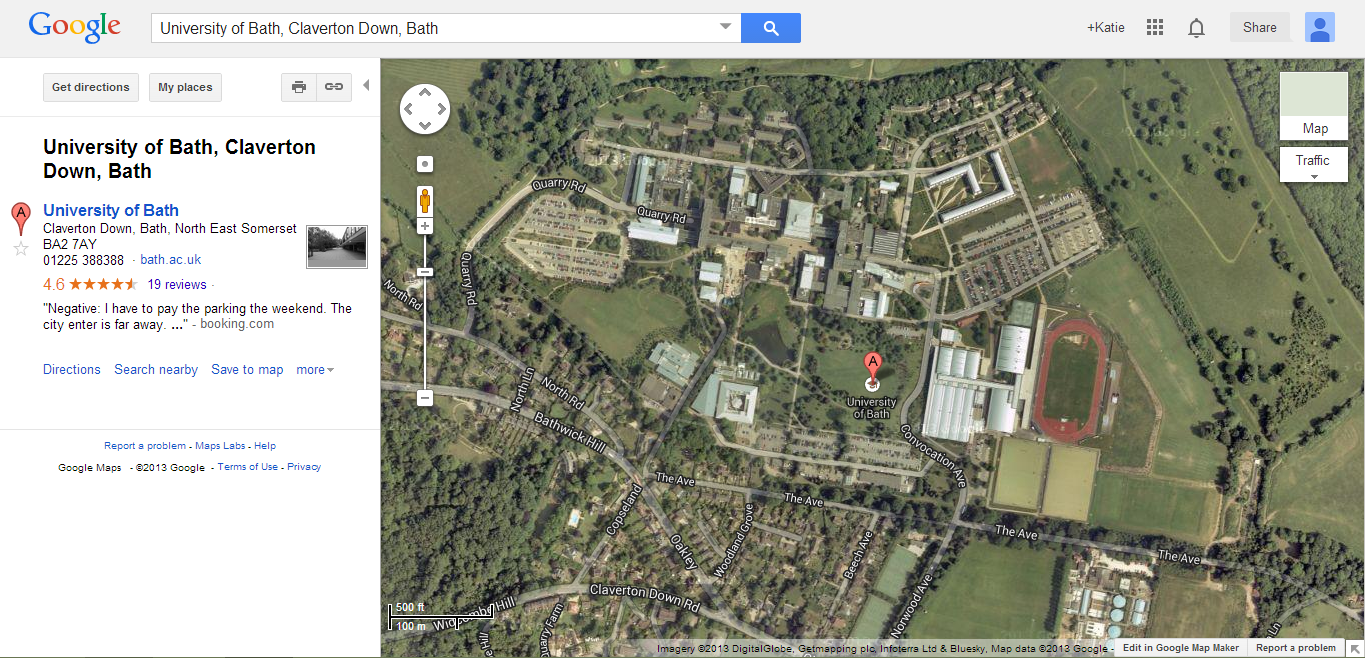
\includegraphics[keepaspectratio, width=\textwidth]{googlemapsexample.png}
 \caption{Google Maps}
\end{figure}

\section*{Users \& significance to those users}
The tool we will be developing will be primarily aimed towards the students of Bath University.  The GPS navigation system will primarily be aimed at new students who do not know their way around the university. And the computer finder will primarily be aimed at students who are not living on campus as they will not be able to easily access a computer whilst on campus. Many of our key features are designed to aid the process of learning by reducing time wasted trying to find a suitable work station on campus. Our focus on the specific user group of students does not limit the use of our system, as the university has many industrial visitors who may not know their way around campus.

We have gathered the incentive to develop our system as all members of the team have been in the position of being lost on campus, and thought that the use of a route planner would be beneficial. In addition to this, as second year students now living off campus, we are finding it increasingly difficult to find computers to do work and would benefit from a system similar to the one we are proposing.  Although there is a web page that tells you if there are computers available, it does not inform you if the room currently in use and it is a laborious process to try and access the information relevant. We are striving to develop an application combines all the key aspects of systems, whilst being simple and easy to use so that the user only needs to use our application to find the relevant information.

\clearpage
\section*{Programme and Methodology}
\subsection*{Overall aims of the project}
After deciding on an idea for a project, the team laid out some goals which we would like to achieve, which are separate from the actual implementation. These should enable us to work effectively in a team, and to demonstrate our skills in software engineering. We can also use these goals at the end of the project to assess our performance, and analyse how well the project has gone.

At the highest level, we aim to create a working application which informs students of the location of free computers around campus, and uses GPS navigation to direct the student to the closest free computer. We aim to do this through the effective use of our design model, as well as user involvement through requirements gathering and also during testing.

Another aim is to improve on the existing systems available to students. We wish to create something that is both more usable and more functional than anything that exists in the same domain. To achieve this, we must first carry out research on the current systems, and interview potential users, to find out what areas we can improve in. More generally, we must find out more about usability and also what are the main components a system needs to make it more usable.
\subsection*{Other features of the application}
\begin{description}
\item[Finding services] \hfill \\
This feature will provide information about various services on campus, such as free computers,
shops, eateries and toilets. To find free computers, we needed real time information regarding the
availability of computers at any current moment. After doing some research we found out that this
information can be obtained from BUCS services website:
http://www.bath.ac.uk/bucs/services/pacs/where.html

Our goal is to extract relevant information regarding free computers from this website, save the
information in a data structure and apply algorithms to find the nearest computer room from user's
current position.

This will be very similar with shops and toilets. The user can select the option, and they will be
provided with the location of the service they require.
\item[Person finder] \hfill \\
The user will have the option for other people to be able to see their location on campus. Then, they
will also be able to see the location of other people who have allowed their location to be seen. This
will allow users to see the location of friends, colleagues or lecturers on campus
\item[Weather widget] \hfill \\
This feature will provide the users with the real time information about the weather on campus.
Lectures and Examinations are re-scheduled and sometimes cancelled due to bad weather
conditions. Such a feature will be very helpful for the students since they can check the weather
status directly from their smart phones. For this feature we need real time information regarding the
weather at any current moment. Our goal is to present this information using the Android weather
widget. One additional feature we are adding to this is the background image of the application will
change automatically depending on the weather conditions.
\end{description}

\begin{table}[H]
% \hspace*{-2cm}
\newcolumntype{S}{>{\small}X}
\newcolumntype{E}{>{\small}c}
\begin{tabularx}{\textwidth}{ |S|S| }
  \hline
  \bf{Objectives and milestones} & \bf{Aim} \\ \hline
  Questionnaires & Initial requirement specification \\ \hline
  Second round of questionnaires based on the results of the first one & Requirement specification \\ \hline
  Feasibility research & Judge implementation feasability based on gathered user input  \\ \hline
  Gather user feedback on the prototype & Get early impressions about the application  \\ \hline
  Interview the users during development & Guide development based on user feedback  \\ \hline
  Analytical and empirical evaluation & Judge the application suitability for the task \\ \hline
\end{tabularx}
\caption{Programme of research work}
\end{table}

For dates, consult the Gantt chart at the end of the document.

\section*{System and programming platforms}
The software platform we are using is Android.  The reason for this is:
\begin{enumerate}
\item{Smartphones are becoming popularised among mobile users, and the largest proportion of them are using Android-based phones.}
\item{Android is open source. Which means it is easier for developers to customize software components and the software can be used on multiple devices.}
\item{Development for Android is easier for developers familiar with Java and all of the team members have learned Java to some extent.}
\item{Compared to iOS and windows phone we don't need to worry about licencing issues and this makes it easier to deliver our application to everyone without cost.}
\end{enumerate}
Android in terms of the objectives of our system
\begin{enumerate}
\item{Android provides a Map API that will make it easier to code and think about system elements such as buildings and shops as objects in the real world.}
\item{Android has a lot of documentation about how to design and manipulate graphical elements. This will make it easier to code the higher level graphical model.}
\item{Android provides a host of efficient data structures which are in-built and do not have to be coded from scratch. (Example: List View, List Adapter, Stacks, Trees etc.)}
\end{enumerate}

\begin{figure}[H]
 \centering
 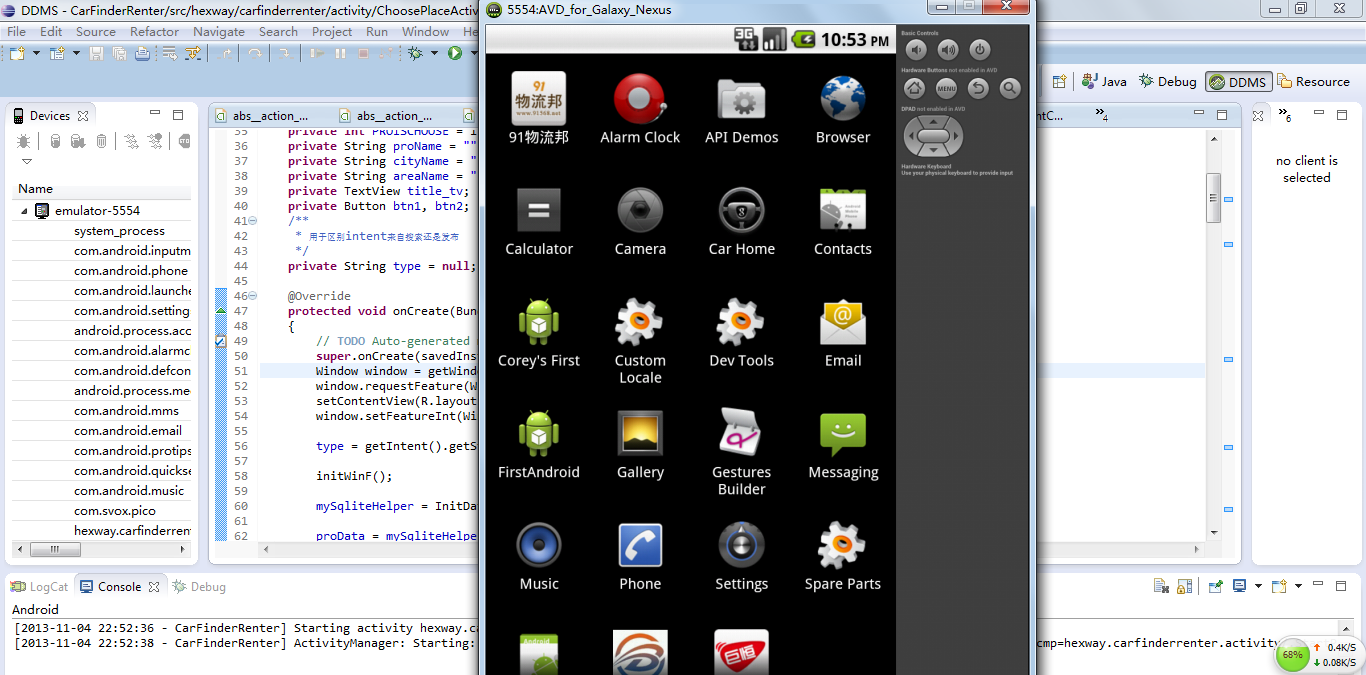
\includegraphics[keepaspectratio, width=\textwidth]{androiddev.png}
 \caption{Android development environment}
\end{figure}

\section*{Work plan}
During the project planning stage, each of our group members were delegated tasks and dealt with problems that came out during the development process.
This is how we approached our project planning:
\begin{enumerate}
\item{We created a Gantt chart allowing us to have an overview of the project process.}
\item{We created a GitHub version control repository to store the files and code for our project.}
\item{We formed a Facebook group that allows us to convey our opinions and ideas to the project instantly.}
\end{enumerate}
In order to keep track of the project, we did the following:
\begin{enumerate}
\item{Our group decided to meet at least once a week to discuss the progress we have made so far.}
\item{We recorded the start and end time of each of our group meetings and documented the entire meeting.}
\end{enumerate}

\begin{figure}[H]
 \centering
 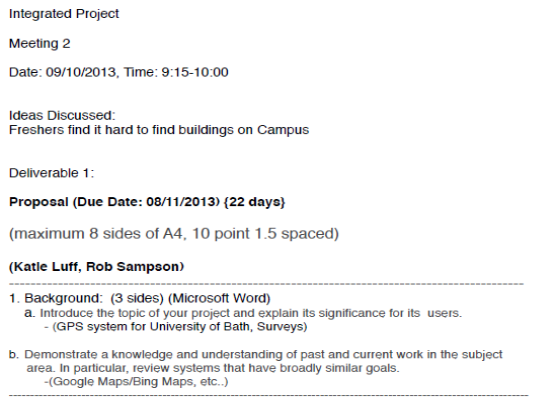
\includegraphics[keepaspectratio, scale=0.5]{meeting.png}
 \caption{Meeting minutes}
\end{figure}

% We put the generated chart on the last page.
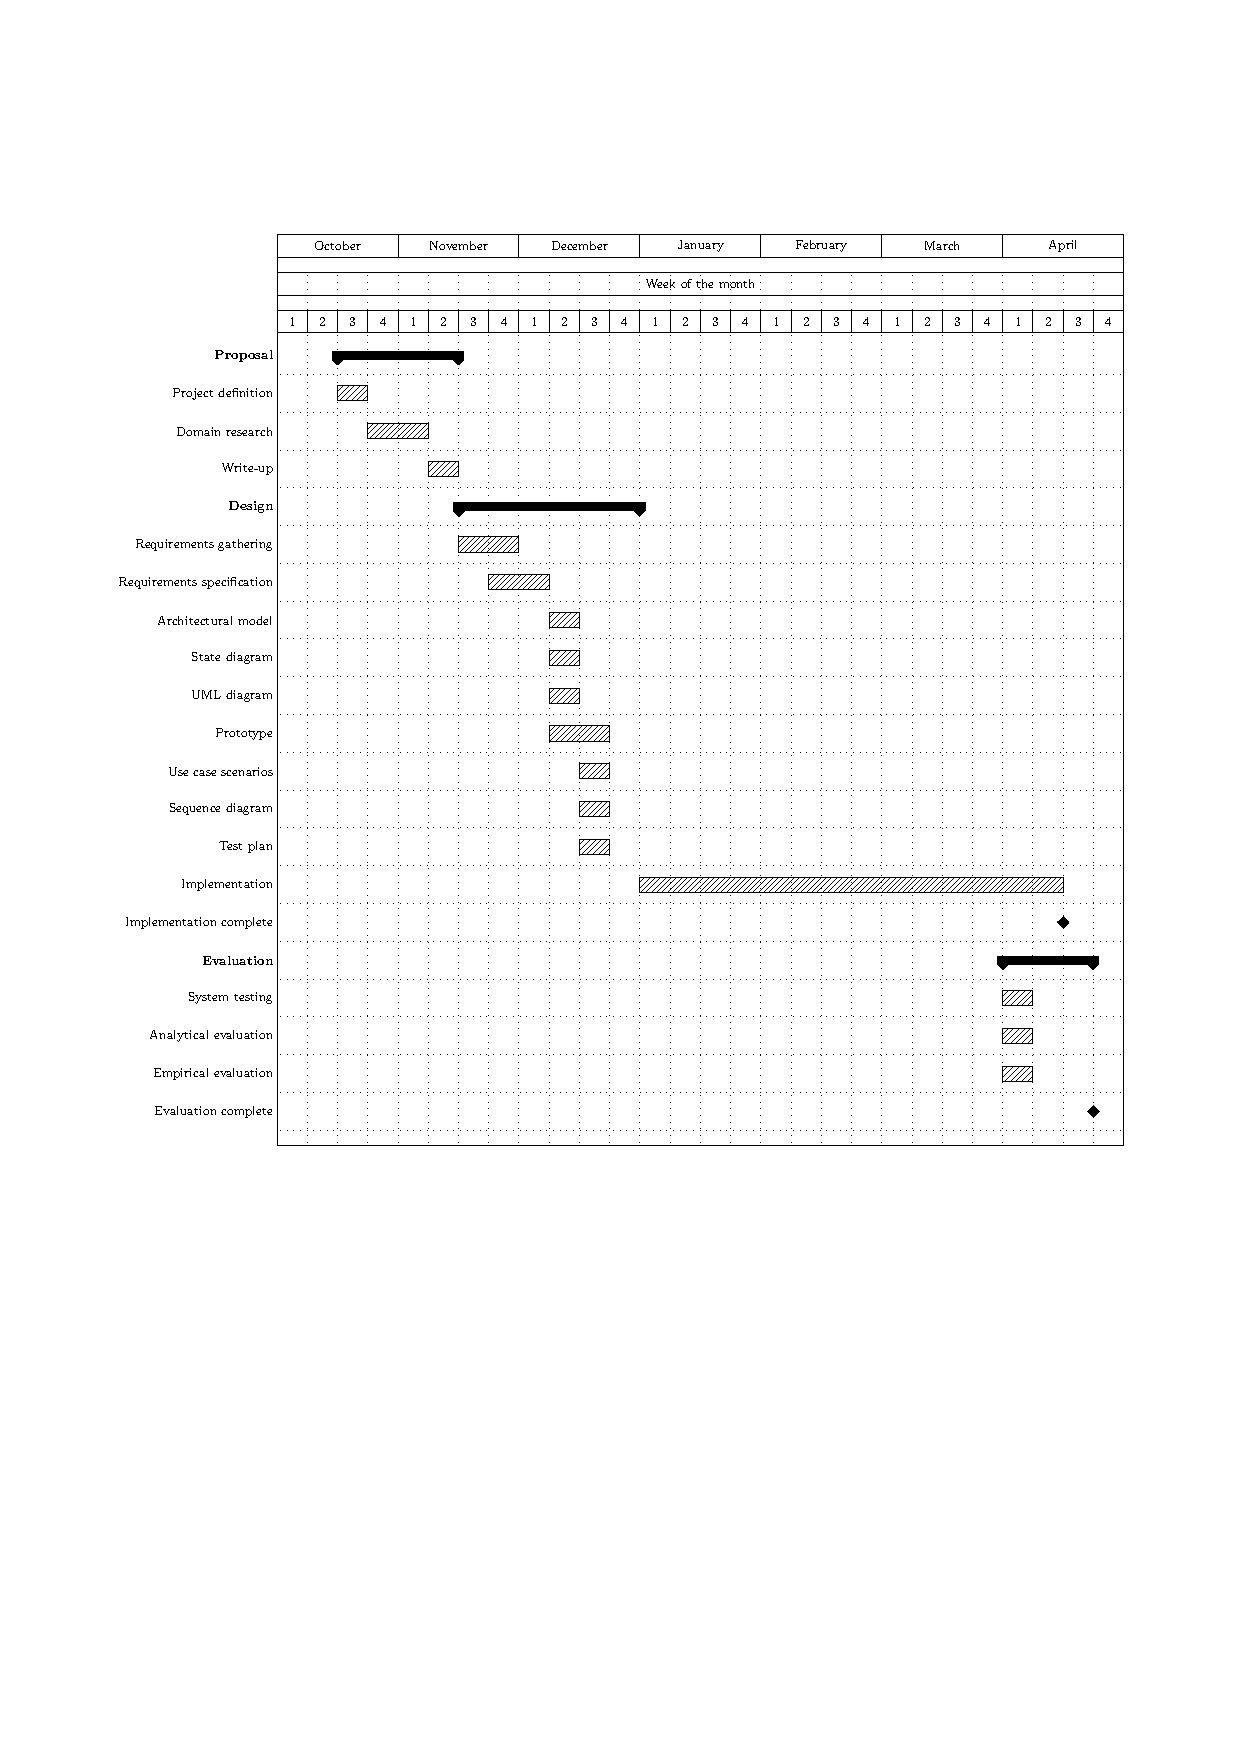
\includepdf[pages={1}]{ganttchart.pdf}

\end{document}
